% Vorgaben Assignment aus Studienheft SQL03
% Formatvorgaben fuer den Text
% Umfang: 8 - 10 Seiten (inkl. Abbildungen und Tabellen, aber ohne Deckblatt, % Gliederung und Literaturverzeichnis, Eidesstattliche Erklaerung)
% Zeilenabstand: 1,5
% Schriftart: frei
% Schriftgrad: 12 pt
% Variablen, physikalische Groessen und Funktionszeichen werden kursiv gedruckt.
% Korrekturrand: links: 4,5 cm, rechts 2,0 cm, oben und unten jeweils 3,0 cm
% Deckblatt: (Adresse, AKAD-E-Mail-Adresse, Immatrikulationsnummer, Modul-
% bezeichnung, Thema, Datum, Felder für Korrektor)
% Gliederung (1 Seite)
% Literaturverzeichnis (3 - 5 Literaturquellen  z. B. Lehrbuecher, aktuelle Fachartikel recherchieren)
% Eidesstattliche Erklaerung (unterschrieben und fest eingebunden)
% Bearbeitungsdauer: 2 Monate


\documentclass[a4paper,12pt]{article}
\usepackage{german}
\usepackage[nottoc]{tocbibind} % Anzeigen des Literaturverzeichnisses im TOC
\usepackage{epsfig}
\usepackage{times}
\usepackage{supertabular}
\usepackage{wrapfig}
\usepackage{multirow}
\usepackage[onehalfspacing]{setspace}
\usepackage{listings}
\usepackage{mathptmx}
\usepackage{geometry}
\usepackage{helvet}
\usepackage{courier}
\usepackage{setspace}
\usepackage{textcomp}
\usepackage[T1]{fontenc}
\usepackage[utf8]{inputenc}
\usepackage{fancyhdr}
\usepackage{float} % Notwendig fuer figure[h]
\usepackage[printonlyused]{acronym}

\newif\iflistoffigures
\newif\iflistoftables
\newif\ifacronym

%Titel
\newcommand*{\Titel}{Thema des Assignments} 

%Betreff
\newcommand*{\Arbeitstyp}{Assignment im Modul ABC01} 

% Akademischer Grad
\newcommand*{\Grad}{Master of Science (M.Sc.)} 

%Betreuer
\newcommand*{\Betreuer}{Prof. Dr. Mustermann} 

%Vor- und Nachname
\newcommand*{\Name}{Max Mustermann}

%Straße und Hausnummer
\newcommand*{\Strasse}{Musterstr. 1a} 

%Plz und Ort
\newcommand*{\PlzOrt}{12345 Musterhausen} 

%Immatrikulationsnummer
\newcommand*{\Immatrikulationsnummer}{123456}

%Bearbeitungszeit
\newcommand*{\Bearbeitungszeit}{8 Wochen}

%Studiengang
\newcommand*{\Studiengang}{IT-Management}

%Email 
\newcommand*{\Email}{max.mustermann@akad.de} 

%PDF Beschreibung
\newcommand*{\pdfsubject}{Eine kurze Beschreibung, worum es geht}

%PDF Keywords
\newcommand*{\pdfkeywords}{akad, assignment, meta, information, pdf, hyperref, latex}


%(Wenn nicht benötigt, Zeile mit % auskommentieren oder löschen)

%% Anhang 
\appendixtrue

%% Verzeichnisse 
%
%% Abbildungsverzeichnis 
\listoffigurestrue
%% Tabellenverzeichnis
\listoftablestrue
%% Abkürzungsverzeichnis
\acronymtrue
%% Formelverzeichnis
%\listofformelntrue

%% Wird Vorlage für Assignment benutzt
\assignmenttrue

\usepackage[
	pdftitle={\Titel},
	pdfsubject={Eine kurze Beschreibung, worum es geht},
	pdfauthor={Max Mustermann},
	pdfkeywords={akad, assignment, meta, information, pdf, hyperref, latex}
	hyperfootnotes=false,
	colorlinks=false,
	linkcolor=black,
	urlcolor=black
]{hyperref}



\renewcommand{\familydefault}{\rmdefault}
\renewcommand{\bflabel}[1]{\normalfont{\normalsize{#1}}\hfill}

\makeatother

\geometry{a4paper, left=45mm, right=20mm, top=30mm, bottom=30mm}
\pagenumbering{roman}

\begin{document}

\begin{center}
\thispagestyle{empty}
\vspace{9cm}

\Huge{\Titel}
\vspace{1cm}
\onehalfspacing

\Large{\Betreff}

\vspace{1cm}
\Large{\Betreuer \\}
\normalsize
\vspace{2cm}

\Name \\ \Strasse \\ \PlzOrt
\\
\vspace{2cm}

\today

Immatrikulationsnummer: \Immatrikulationsnummer

\href{mailto:\Email}{\Email}
\vspace{3cm}


\includegraphics[scale=0.35]{akad_logo.png}

\end{center}

\clearpage

\normalsize


\begin{spacing}{1.0} % Verzeichnisse werden mit einzeiligem Abstand gesetzt
\newpage

% Inhaltsverzeichnis
\tableofcontents 
\newpage

% Abbildungsverzeichnis
\iflistoffigures
\listoffigures 
\newpage
\fi

% Tabellenverzeichnis
\iflistoftables
\listoftables 
\newpage
\fi

% Abkürzungsverzeichnis
\ifacronym
\chapter*{Abkürzungsverzeichnis}
\addcontentsline{toc}{chapter}{Abkürzungsverzeichnis} 


%% Hier Abkürzungen angeben
\begin{acronym}[ABK]
	\acro{Abk}{Abkürzungen}
	\acro{Test}{Wird nicht im Text verwendet und taucht auch nicht im Verzeichnis auf}
\end{acronym}

\fi

\end{spacing} 

\clearpage

\newcounter{romanPagenumber} 
\setcounter{romanPagenumber}{\value{page}} % Roemische Seitenanzahl speichern.


\pagestyle{fancy}
\fancyhead{}
\fancyhead[LO,RE]{\textsc{\Titel}}
\fancyhead[RO,LE]{\thepage}
\fancyfoot[CO,CE]{}

\nocite{*} 

\pagenumbering{arabic}

\begin{spacing}{1.5} % Zeilenabstand: 1,5 fuer den Textteil

\chapter{Einleitung}
\section{Einführung in das Thema}
Lorem ipsum dolor sit amet, consetetur sadipscing elitr, sed diam nonumy eirmod tempor invidunt ut labore et dolore magna aliquyam erat, sed diam voluptua. At vero eos et accusam et justo duo dolores et ea rebum. Stet clita kasd gubergren, no sea takimata sanctus est Lorem ipsum dolor sit amet. Lorem ipsum dolor sit amet, consetetur sadipscing elitr, sed diam nonumy eirmod tempor invidunt ut labore et dolore magna aliquyam erat, sed diam voluptua. At vero eos et accusam et justo duo dolores et ea rebum. Stet clita kasd gubergren, no sea takimata sanctus est Lorem ipsum dolor sit amet.

\section{Problemstellung und Ziel dieser Arbeit}

Lorem ipsum dolor sit amet, consetetur sadipscing elitr, sed diam nonumy eirmod tempor invidunt ut labore et dolore magna aliquyam erat, sed diam voluptua. At vero eos et accusam et justo duo dolores et ea rebum. Stet clita kasd gubergren, no sea takimata sanctus est Lorem ipsum dolor sit amet. Lorem ipsum dolor sit amet, consetetur sadipscing elitr, sed diam nonumy eirmod tempor invidunt ut labore et dolore magna aliquyam erat, sed diam voluptua. At vero eos et accusam et justo duo dolores et ea rebum. Stet clita kasd gubergren, no sea takimata sanctus est Lorem ipsum dolor sit amet.

\section{Aufbau der Arbeit}

\todo{An die fertige Arbeit anpassen}

Lorem ipsum dolor sit amet, consetetur sadipscing elitr, sed diam nonumy eirmod tempor invidunt ut labore et dolore magna aliquyam erat, sed diam voluptua. At vero eos et accusam et justo duo dolores et ea rebum. Stet clita kasd gubergren, no sea takimata sanctus est Lorem ipsum dolor sit amet. Lorem ipsum dolor sit amet, consetetur sadipscing elitr, sed diam nonumy eirmod tempor invidunt ut labore et dolore magna aliquyam erat, sed diam voluptua. 



\section{Grundlagen}
\subsection{Text}

\subsubsection{Fett}
\textbf{Lorem ipsum dolor sit amet, consetetur sadipscing elitr, sed diam nonumy eirmod tempor invidunt ut labore et dolore magna aliquyam erat, sed diam voluptua.}

\subsubsection{Kursiv}
\textit{Lorem ipsum dolor sit amet, consetetur sadipscing elitr, sed diam nonumy eirmod tempor invidunt ut labore et dolore magna aliquyam erat, sed diam voluptua.}

\subsubsection{Unterstrichen}
orem ipsum \underline{dolor} sit amet, consetetur sadipscing elitr, sed diam nonumy eirmod \underline{tempor} invidunt ut labore et dolore magna \underline{aliquyam} erat, sed diam voluptua.

\subsection{Fußnote}

Text mit Fußnote \footnote{Die Fußnote zum Text} 

\subsection{Zitate}

Dies ist ein ganz kurzer Beispieltext \footnote{\cite{Baeumle-Courth2004}}. Und noch ein weites Zitat \footnote{\cite{Torvalds2001}}
\\
Zitate auf Webseiten \footnote{\cite{gabler:individualsoftware}} \footnote{\cite{gabler:standardsoftware}}
\\
http://www.literatur-generator.de/

\subsection{Aufzählung}

\begin{itemize}
\item\textit{Punkt 1:} Text
\item Punkt 2: Text
\item Punkt 3: \\ Text
\end{itemize}

\subsection{Abkürzungen}
Hier werden \ac{Abk} aus dem Verzeichnis aufgerufen und gleich nochmal die gleiche \ac{Abk}.


\section{Hauptteil}

\subsection{Tabelle}

\begin{center}
\tablehead{ \textbf{Head1} & \textbf{Head2} & \textbf{Head3}
\\ }
\bottomcaption[Beschreibung]{Beschreibung. Quelle: Berger, Vorlesung, 2012, München }
\begin{supertabular}{c|c|c}
\hline
1 & 2 & 3 \\
4 & 5 & 6 \\
7 & 8 & 9 \\
1 & 2 & 3 \\
4 & 5 & 6 \\
7 & 8 & 9 \\
\end{supertabular}
\end{center}

\subsection{Bilder}

\begin{figure}[H]
\begin{center}
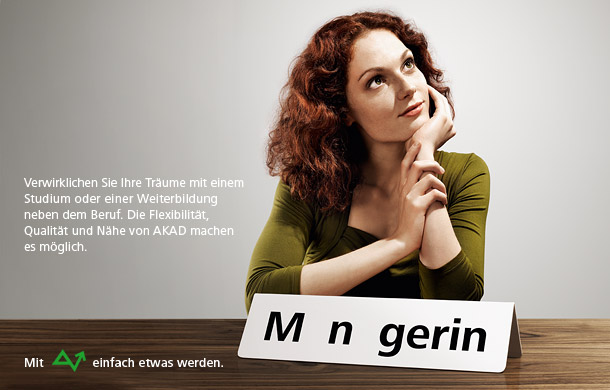
\includegraphics[scale=0.5]{akad_bild1.jpg}
\caption[Akad]{Akad. Quelle: www.akad.de}
\end{center}
\end{figure}

%%Einkommentieren fuer Syntax Highlighting. In vorlage.tex muessen auch 2 Zeilen einkommentiert werden
%\subsection{Syntax Highlighting}
%\begin{figure}[h]
%\begin{minted}[linenos=true,bgcolor=bg]{php}
%<?php 
%$title="Lorem";
%$desc = "Lorem Ipsum";
%include($_SERVER['DOCUMENT_ROOT'].'/header.php'); 
%?>
%\end{minted}
%\caption{Quellcode: Aufruf von header.php (PHP)}
%\label{abb:header}
%\end{figure}

\subsection{Formeln}

\begin{Formel}
$a+b=c$
\caption{AB Formel}
\end{Formel}





\chapter{Bewertung}

\section{Zusammenfassung}
Lorem ipsum dolor sit amet, consetetur sadipscing elitr, sed diam nonumy eirmod tempor invidunt ut labore et dolore magna aliquyam erat, sed diam voluptua. At vero eos et accusam et justo duo dolores et ea rebum. Stet clita kasd gubergren, no sea takimata sanctus est Lorem ipsum dolor sit amet.

\section{kritische Würdigung}
Lorem ipsum dolor sit amet, consetetur sadipscing elitr, sed diam nonumy eirmod tempor invidunt ut labore et dolore magna aliquyam erat, sed diam voluptua. At vero eos et accusam et justo duo dolores et ea rebum. Stet clita kasd gubergren, no sea takimata sanctus est Lorem ipsum dolor sit amet.

\section{Ausblick}
Lorem ipsum dolor sit amet, consetetur sadipscing elitr, sed diam nonumy eirmod tempor invidunt ut labore et dolore magna aliquyam erat, sed diam voluptua. At vero eos et accusam et justo duo dolores et ea rebum. Stet clita kasd gubergren, no sea takimata sanctus est Lorem ipsum dolor sit amet.

\section{Erfolgsfaktoren}
Lorem ipsum dolor sit amet, consetetur sadipscing elitr, sed diam nonumy eirmod tempor invidunt ut labore et dolore magna aliquyam erat, sed diam voluptua. At vero eos et accusam et justo duo dolores et ea rebum. Stet clita kasd gubergren, no sea takimata sanctus est Lorem ipsum dolor sit amet.

\end{spacing}

\clearpage

% Literaturverzeichniss - Ab hier wieder Roemische Seitenzahlen
\pagestyle{plain}
\pagenumbering{roman}
\setcounter{page}{\theromanPagenumber}
\bibliographystyle{apalike}
\bibliography{literatur}
\onehalfspacing
\clearpage

\pagestyle{empty} 
\thispagestyle{empty}

\begin{center}
{\Large Eidesstattliche Erkl"arung}
\vspace*{4cm}\end{center}
\noindent
Ich versichere, dass ich das beiliegende Assignment selbstst"andig verfasst, keine anderen als die angegebenen Quellen und Hilfsmittel benutzt sowie alle w"ortlich oder sinngem"a"s "ubernommenen Stellen in der Arbeit gekennzeichnet habe. 
\vspace{3cm}

\hspace{-0.8cm}
\rule[0.5ex]{6.5cm}{1pt}
\hspace{1.3cm}
\rule[0.5ex]{6.5cm}{1pt}
(Datum, Ort)
\hspace{6.3cm}(Unterschrift)

\clearpage

%Messbox zur Druckkontrolle:
\newcommand{\Messbox}[2]{% Parameters: #1=Breite, #2=Hoehe
\setlength{\unitlength}{1.0mm}%
\begin{picture}(#1,#2)%
\linethickness{0.05mm}%
\put(0,0){\dashbox{0.2}(#1,#2)%
{\parbox{#1mm}{%
\centering\footnotesize 
%{\bf MESSBOX}\\ 
Breite $ = #1 {\rm\ mm}$\\
H\"ohe $ = #2 {\rm\ mm}$
}}}\end{picture}
}

\begin{center}
\textbf{--- Druckgröße kontrollieren! ---}
\\
\Messbox{100}{50} % Angabe der Breite/Hoehe in mm
\\
\textbf{--- Diese Seite nach dem Druck entfernen! ---}
\end{center}


\end{document}

